%%%%%%%%%%%%%%%%%%%%%%%%%%%%%%%%%%%%%%%%%%%%%%%%%%%%%%%%%%%%%%%%%%%%%%
% This layout was adapted from one found at latextemplates.com which
% was adapted from another.
%
% License: CC BY-NC-SA 3.0
% (http://creativecommons.org/licenses/by-nc-sa/3.0/)
%
% Original header:
%
% This is a LaTeX version of the sample laboratory report from
% Virginia Tech's copyrighted 08-09 CHEM 1045/1046 lab manual.
% Reproduction of this one appendix section for academic purposes
% should fall under fair use.
%
%%%%%%%%%%%%%%%%%%%%%%%%%%%%%%%%%%%%%%%%%%%%%%%%%%%%%%%%%%%%%%%%%%%%%%

\documentclass{article}

\usepackage{graphicx}
%\usepackage[acronym]{glossaries} % Lets us use acronyms
\usepackage{siunitx} % SI units in math mode

\author{}
\title{ELEC-313 \\ Lab 2: Diode Characterization \\ }
\date{\today}

%\loadglsentries{acronyms} % Actually loads 'acronyms.tex'
%\makeglossaries

\begin{document}

\maketitle

\begin{center}
  \begin{tabular}{lr}
    Date Performed: & September 18, 2013 \\
    Partners: & Charles Pittman \\
    & Stephen Wilson \\
  \end{tabular}
\end{center}

\pagebreak

% Removes indentation from paragraphs: \setlength\parindent{0pt}

% Number the enumerate environment (unordered lists) by letter:
\renewcommand{\labelenumi}{\alph{enumi}.}

\section{Objective}
\label{sec:objective}

The objective is to observe the basic operation of a diode.  In
addition, the Schlockley equation (Eq~\ref{eqn:schlockley}) is used to
find the diode's reverse saturation current ($I_S$) and thermal
voltage ($V_T$) using measured values in the lab.

\section{Equipment}
\label{sec:equipment}

\begin{tabular}{ll}
  \centering
  Diode: 1N4002 & Power supply: HP E3631A \\
  Resistors: \SI{330}{\ohm}, \SI{470}{\ohm}, \SI{680}{\ohm} & Multimeter: Fluke 8010A \\
  Resistive decade box: HeathKit IN-3117 & \\
\end{tabular}

\section{Schematics}
\label{sec:schematics}

\subsection{Circuits Tested}
\label{sec:ckt_tested}

\begin{figure}[hbtp]
  \centering
  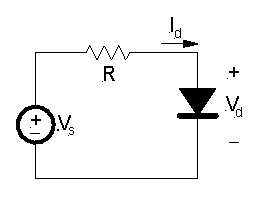
\includegraphics[]{img/circuit1}
  \caption{\label{fig:circuit1} Circuit used for Part A and Part B.}
\end{figure}

\begin{figure}[hbtp]
  \centering
  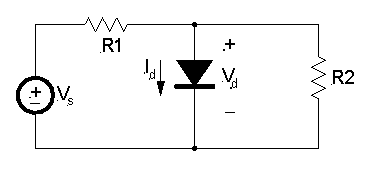
\includegraphics[]{img/circuit2}
  \caption{\label{fig:circuit2} Circuit used for Part C.}
\end{figure}

\section{Procedure}
\label{sec:procedure}

\subsection{Part A}
\label{sec:proc_a}

The circuit in Figure~\ref{fig:circuit1} with $R = \SI{470}{\ohm}$ and
the power supply as $V_S$.

\subsection{Part B}
\label{sec:proc_b}

Lorem ipsum dolor sit amet, consectetuer adipiscing elit. Donec
hendrerit tempor tellus. Donec pretium posuere tellus. Proin quam
nisl, tincidunt et, mattis eget, convallis nec, purus. Cum sociis
natoque penatibus et magnis dis parturient montes, nascetur ridiculus
mus. Nulla posuere. Donec vitae dolor. Nullam tristique diam non
turpis. Cras placerat accumsan nulla. Nullam rutrum. Nam vestibulum
accumsan nisl.

\subsection{Part C}
\label{sec:proc_c}

Lorem ipsum dolor sit amet, consectetuer adipiscing elit. Donec
hendrerit tempor tellus. Donec pretium posuere tellus. Proin quam
nisl, tincidunt et, mattis eget, convallis nec, purus. Cum sociis
natoque penatibus et magnis dis parturient montes, nascetur ridiculus
mus. Nulla posuere. Donec vitae dolor. Nullam tristique diam non
turpis. Cras placerat accumsan nulla. Nullam rutrum. Nam vestibulum
accumsan nisl.

\section{Results}
\label{sec:results}

\subsection{Part A}
\label{sec:result_a}

\begin{figure}[hbtp]
  \centering
  % GNUPLOT: LaTeX picture
\setlength{\unitlength}{0.240900pt}
\ifx\plotpoint\undefined\newsavebox{\plotpoint}\fi
\begin{picture}(1500,900)(0,0)
\sbox{\plotpoint}{\rule[-0.200pt]{0.400pt}{0.400pt}}%
\put(151.0,131.0){\rule[-0.200pt]{4.818pt}{0.400pt}}
\put(131,131){\makebox(0,0)[r]{ 0}}
\put(1419.0,131.0){\rule[-0.200pt]{4.818pt}{0.400pt}}
\put(151.0,196.0){\rule[-0.200pt]{4.818pt}{0.400pt}}
\put(131,196){\makebox(0,0)[r]{ 2}}
\put(1419.0,196.0){\rule[-0.200pt]{4.818pt}{0.400pt}}
\put(151.0,260.0){\rule[-0.200pt]{4.818pt}{0.400pt}}
\put(131,260){\makebox(0,0)[r]{ 4}}
\put(1419.0,260.0){\rule[-0.200pt]{4.818pt}{0.400pt}}
\put(151.0,325.0){\rule[-0.200pt]{4.818pt}{0.400pt}}
\put(131,325){\makebox(0,0)[r]{ 6}}
\put(1419.0,325.0){\rule[-0.200pt]{4.818pt}{0.400pt}}
\put(151.0,389.0){\rule[-0.200pt]{4.818pt}{0.400pt}}
\put(131,389){\makebox(0,0)[r]{ 8}}
\put(1419.0,389.0){\rule[-0.200pt]{4.818pt}{0.400pt}}
\put(151.0,454.0){\rule[-0.200pt]{4.818pt}{0.400pt}}
\put(131,454){\makebox(0,0)[r]{ 10}}
\put(1419.0,454.0){\rule[-0.200pt]{4.818pt}{0.400pt}}
\put(151.0,518.0){\rule[-0.200pt]{4.818pt}{0.400pt}}
\put(131,518){\makebox(0,0)[r]{ 12}}
\put(1419.0,518.0){\rule[-0.200pt]{4.818pt}{0.400pt}}
\put(151.0,583.0){\rule[-0.200pt]{4.818pt}{0.400pt}}
\put(131,583){\makebox(0,0)[r]{ 14}}
\put(1419.0,583.0){\rule[-0.200pt]{4.818pt}{0.400pt}}
\put(151.0,647.0){\rule[-0.200pt]{4.818pt}{0.400pt}}
\put(131,647){\makebox(0,0)[r]{ 16}}
\put(1419.0,647.0){\rule[-0.200pt]{4.818pt}{0.400pt}}
\put(151.0,712.0){\rule[-0.200pt]{4.818pt}{0.400pt}}
\put(131,712){\makebox(0,0)[r]{ 18}}
\put(1419.0,712.0){\rule[-0.200pt]{4.818pt}{0.400pt}}
\put(151.0,776.0){\rule[-0.200pt]{4.818pt}{0.400pt}}
\put(131,776){\makebox(0,0)[r]{ 20}}
\put(1419.0,776.0){\rule[-0.200pt]{4.818pt}{0.400pt}}
\put(151.0,131.0){\rule[-0.200pt]{0.400pt}{4.818pt}}
\put(151,90){\makebox(0,0){ 0}}
\put(151.0,756.0){\rule[-0.200pt]{0.400pt}{4.818pt}}
\put(323.0,131.0){\rule[-0.200pt]{0.400pt}{4.818pt}}
\put(323,90){\makebox(0,0){ 0.1}}
\put(323.0,756.0){\rule[-0.200pt]{0.400pt}{4.818pt}}
\put(494.0,131.0){\rule[-0.200pt]{0.400pt}{4.818pt}}
\put(494,90){\makebox(0,0){ 0.2}}
\put(494.0,756.0){\rule[-0.200pt]{0.400pt}{4.818pt}}
\put(666.0,131.0){\rule[-0.200pt]{0.400pt}{4.818pt}}
\put(666,90){\makebox(0,0){ 0.3}}
\put(666.0,756.0){\rule[-0.200pt]{0.400pt}{4.818pt}}
\put(838.0,131.0){\rule[-0.200pt]{0.400pt}{4.818pt}}
\put(838,90){\makebox(0,0){ 0.4}}
\put(838.0,756.0){\rule[-0.200pt]{0.400pt}{4.818pt}}
\put(1010.0,131.0){\rule[-0.200pt]{0.400pt}{4.818pt}}
\put(1010,90){\makebox(0,0){ 0.5}}
\put(1010.0,756.0){\rule[-0.200pt]{0.400pt}{4.818pt}}
\put(1181.0,131.0){\rule[-0.200pt]{0.400pt}{4.818pt}}
\put(1181,90){\makebox(0,0){ 0.6}}
\put(1181.0,756.0){\rule[-0.200pt]{0.400pt}{4.818pt}}
\put(1353.0,131.0){\rule[-0.200pt]{0.400pt}{4.818pt}}
\put(1353,90){\makebox(0,0){ 0.7}}
\put(1353.0,756.0){\rule[-0.200pt]{0.400pt}{4.818pt}}
\put(151.0,131.0){\rule[-0.200pt]{0.400pt}{155.380pt}}
\put(151.0,131.0){\rule[-0.200pt]{310.279pt}{0.400pt}}
\put(1439.0,131.0){\rule[-0.200pt]{0.400pt}{155.380pt}}
\put(151.0,776.0){\rule[-0.200pt]{310.279pt}{0.400pt}}
\put(30,453){\makebox(0,0){\shortstack{$I_d$\\(mA)}}}
\put(795,29){\makebox(0,0){$V_d$ (V)}}
\put(795,838){\makebox(0,0){Diode Current vs. Voltage}}
\put(171,756){\usebox{\plotpoint}}
\put(171.0,756.0){\rule[-0.200pt]{33.726pt}{0.400pt}}
\put(311,756){\usebox{\plotpoint}}
\put(171.0,756.0){\rule[-0.200pt]{33.726pt}{0.400pt}}
\put(627,131){\makebox(0,0){$+$}}
\put(587,131){\makebox(0,0){$+$}}
\put(943,134){\makebox(0,0){$+$}}
\put(1071,146){\makebox(0,0){$+$}}
\put(1130,161){\makebox(0,0){$+$}}
\put(1166,176){\makebox(0,0){$+$}}
\put(1192,192){\makebox(0,0){$+$}}
\put(1212,208){\makebox(0,0){$+$}}
\put(1228,225){\makebox(0,0){$+$}}
\put(1242,241){\makebox(0,0){$+$}}
\put(1254,257){\makebox(0,0){$+$}}
\put(1264,274){\makebox(0,0){$+$}}
\put(1272,291){\makebox(0,0){$+$}}
\put(1281,307){\makebox(0,0){$+$}}
\put(1288,324){\makebox(0,0){$+$}}
\put(1295,341){\makebox(0,0){$+$}}
\put(1302,358){\makebox(0,0){$+$}}
\put(1307,374){\makebox(0,0){$+$}}
\put(1312,392){\makebox(0,0){$+$}}
\put(1317,408){\makebox(0,0){$+$}}
\put(1322,425){\makebox(0,0){$+$}}
\put(1331,459){\makebox(0,0){$+$}}
\put(1339,493){\makebox(0,0){$+$}}
\put(1346,528){\makebox(0,0){$+$}}
\put(1351,562){\makebox(0,0){$+$}}
\put(1358,596){\makebox(0,0){$+$}}
\put(1363,631){\makebox(0,0){$+$}}
\put(1369,665){\makebox(0,0){$+$}}
\put(1374,701){\makebox(0,0){$+$}}
\put(1377,736){\makebox(0,0){$+$}}
\put(1382,771){\makebox(0,0){$+$}}
\put(151.0,131.0){\rule[-0.200pt]{0.400pt}{155.380pt}}
\put(151.0,131.0){\rule[-0.200pt]{310.279pt}{0.400pt}}
\put(1439.0,131.0){\rule[-0.200pt]{0.400pt}{155.380pt}}
\put(151.0,776.0){\rule[-0.200pt]{310.279pt}{0.400pt}}
\end{picture}

  \caption{\label{fig:part_a_graph} Diode characteristics measured in Part A.}
\end{figure}

\begin{figure}[hbtp]
  \centering
  % GNUPLOT: LaTeX picture
\setlength{\unitlength}{0.240900pt}
\ifx\plotpoint\undefined\newsavebox{\plotpoint}\fi
\sbox{\plotpoint}{\rule[-0.200pt]{0.400pt}{0.400pt}}%
\begin{picture}(1500,900)(0,0)
\sbox{\plotpoint}{\rule[-0.200pt]{0.400pt}{0.400pt}}%
\put(171.0,131.0){\rule[-0.200pt]{4.818pt}{0.400pt}}
\put(151,131){\makebox(0,0)[r]{ 0}}
\put(1419.0,131.0){\rule[-0.200pt]{4.818pt}{0.400pt}}
\put(171.0,239.0){\rule[-0.200pt]{4.818pt}{0.400pt}}
\put(151,239){\makebox(0,0)[r]{ 0.5}}
\put(1419.0,239.0){\rule[-0.200pt]{4.818pt}{0.400pt}}
\put(171.0,346.0){\rule[-0.200pt]{4.818pt}{0.400pt}}
\put(151,346){\makebox(0,0)[r]{ 1}}
\put(1419.0,346.0){\rule[-0.200pt]{4.818pt}{0.400pt}}
\put(171.0,454.0){\rule[-0.200pt]{4.818pt}{0.400pt}}
\put(151,454){\makebox(0,0)[r]{ 1.5}}
\put(1419.0,454.0){\rule[-0.200pt]{4.818pt}{0.400pt}}
\put(171.0,561.0){\rule[-0.200pt]{4.818pt}{0.400pt}}
\put(151,561){\makebox(0,0)[r]{ 2}}
\put(1419.0,561.0){\rule[-0.200pt]{4.818pt}{0.400pt}}
\put(171.0,669.0){\rule[-0.200pt]{4.818pt}{0.400pt}}
\put(151,669){\makebox(0,0)[r]{ 2.5}}
\put(1419.0,669.0){\rule[-0.200pt]{4.818pt}{0.400pt}}
\put(171.0,776.0){\rule[-0.200pt]{4.818pt}{0.400pt}}
\put(151,776){\makebox(0,0)[r]{ 3}}
\put(1419.0,776.0){\rule[-0.200pt]{4.818pt}{0.400pt}}
\put(171.0,131.0){\rule[-0.200pt]{0.400pt}{4.818pt}}
\put(171,90){\makebox(0,0){ 0}}
\put(171.0,756.0){\rule[-0.200pt]{0.400pt}{4.818pt}}
\put(330.0,131.0){\rule[-0.200pt]{0.400pt}{4.818pt}}
\put(330,90){\makebox(0,0){ 0.1}}
\put(330.0,756.0){\rule[-0.200pt]{0.400pt}{4.818pt}}
\put(488.0,131.0){\rule[-0.200pt]{0.400pt}{4.818pt}}
\put(488,90){\makebox(0,0){ 0.2}}
\put(488.0,756.0){\rule[-0.200pt]{0.400pt}{4.818pt}}
\put(647.0,131.0){\rule[-0.200pt]{0.400pt}{4.818pt}}
\put(647,90){\makebox(0,0){ 0.3}}
\put(647.0,756.0){\rule[-0.200pt]{0.400pt}{4.818pt}}
\put(805.0,131.0){\rule[-0.200pt]{0.400pt}{4.818pt}}
\put(805,90){\makebox(0,0){ 0.4}}
\put(805.0,756.0){\rule[-0.200pt]{0.400pt}{4.818pt}}
\put(964.0,131.0){\rule[-0.200pt]{0.400pt}{4.818pt}}
\put(964,90){\makebox(0,0){ 0.5}}
\put(964.0,756.0){\rule[-0.200pt]{0.400pt}{4.818pt}}
\put(1122.0,131.0){\rule[-0.200pt]{0.400pt}{4.818pt}}
\put(1122,90){\makebox(0,0){ 0.6}}
\put(1122.0,756.0){\rule[-0.200pt]{0.400pt}{4.818pt}}
\put(1281.0,131.0){\rule[-0.200pt]{0.400pt}{4.818pt}}
\put(1281,90){\makebox(0,0){ 0.7}}
\put(1281.0,756.0){\rule[-0.200pt]{0.400pt}{4.818pt}}
\put(1439.0,131.0){\rule[-0.200pt]{0.400pt}{4.818pt}}
\put(1439,90){\makebox(0,0){ 0.8}}
\put(1439.0,756.0){\rule[-0.200pt]{0.400pt}{4.818pt}}
\put(171.0,131.0){\rule[-0.200pt]{0.400pt}{155.380pt}}
\put(171.0,131.0){\rule[-0.200pt]{305.461pt}{0.400pt}}
\put(1439.0,131.0){\rule[-0.200pt]{0.400pt}{155.380pt}}
\put(171.0,776.0){\rule[-0.200pt]{305.461pt}{0.400pt}}
\put(30,453){\makebox(0,0){ln($I_d$) (mA)}}
\put(805,29){\makebox(0,0){$V_d$ (V)}}
\put(805,838){\makebox(0,0){Diode Natural Logarithm of Current vs. Voltage}}
\multiput(1081.58,131.00)(0.497,1.343){51}{\rule{0.120pt}{1.167pt}}
\multiput(1080.17,131.00)(27.000,69.579){2}{\rule{0.400pt}{0.583pt}}
\multiput(1108.58,203.00)(0.496,1.366){45}{\rule{0.120pt}{1.183pt}}
\multiput(1107.17,203.00)(24.000,62.544){2}{\rule{0.400pt}{0.592pt}}
\multiput(1132.58,268.00)(0.495,1.330){35}{\rule{0.119pt}{1.153pt}}
\multiput(1131.17,268.00)(19.000,47.608){2}{\rule{0.400pt}{0.576pt}}
\multiput(1151.58,318.00)(0.494,1.525){25}{\rule{0.119pt}{1.300pt}}
\multiput(1150.17,318.00)(14.000,39.302){2}{\rule{0.400pt}{0.650pt}}
\multiput(1165.58,360.00)(0.492,1.487){21}{\rule{0.119pt}{1.267pt}}
\multiput(1164.17,360.00)(12.000,32.371){2}{\rule{0.400pt}{0.633pt}}
\multiput(1177.58,395.00)(0.492,1.272){21}{\rule{0.119pt}{1.100pt}}
\multiput(1176.17,395.00)(12.000,27.717){2}{\rule{0.400pt}{0.550pt}}
\multiput(1189.59,425.00)(0.489,1.485){15}{\rule{0.118pt}{1.256pt}}
\multiput(1188.17,425.00)(9.000,23.394){2}{\rule{0.400pt}{0.628pt}}
\multiput(1198.59,451.00)(0.488,1.550){13}{\rule{0.117pt}{1.300pt}}
\multiput(1197.17,451.00)(8.000,21.302){2}{\rule{0.400pt}{0.650pt}}
\multiput(1206.59,475.00)(0.488,1.352){13}{\rule{0.117pt}{1.150pt}}
\multiput(1205.17,475.00)(8.000,18.613){2}{\rule{0.400pt}{0.575pt}}
\multiput(1214.59,496.00)(0.482,1.756){9}{\rule{0.116pt}{1.433pt}}
\multiput(1213.17,496.00)(6.000,17.025){2}{\rule{0.400pt}{0.717pt}}
\multiput(1220.59,516.00)(0.485,1.332){11}{\rule{0.117pt}{1.129pt}}
\multiput(1219.17,516.00)(7.000,15.658){2}{\rule{0.400pt}{0.564pt}}
\multiput(1227.59,534.00)(0.482,1.395){9}{\rule{0.116pt}{1.167pt}}
\multiput(1226.17,534.00)(6.000,13.579){2}{\rule{0.400pt}{0.583pt}}
\multiput(1233.59,550.00)(0.477,1.712){7}{\rule{0.115pt}{1.380pt}}
\multiput(1232.17,550.00)(5.000,13.136){2}{\rule{0.400pt}{0.690pt}}
\multiput(1238.60,566.00)(0.468,1.943){5}{\rule{0.113pt}{1.500pt}}
\multiput(1237.17,566.00)(4.000,10.887){2}{\rule{0.400pt}{0.750pt}}
\multiput(1242.59,580.00)(0.477,1.489){7}{\rule{0.115pt}{1.220pt}}
\multiput(1241.17,580.00)(5.000,11.468){2}{\rule{0.400pt}{0.610pt}}
\multiput(1247.59,594.00)(0.477,1.267){7}{\rule{0.115pt}{1.060pt}}
\multiput(1246.17,594.00)(5.000,9.800){2}{\rule{0.400pt}{0.530pt}}
\multiput(1252.59,606.00)(0.488,1.550){13}{\rule{0.117pt}{1.300pt}}
\multiput(1251.17,606.00)(8.000,21.302){2}{\rule{0.400pt}{0.650pt}}
\multiput(1260.59,630.00)(0.488,1.352){13}{\rule{0.117pt}{1.150pt}}
\multiput(1259.17,630.00)(8.000,18.613){2}{\rule{0.400pt}{0.575pt}}
\multiput(1268.59,651.00)(0.482,1.756){9}{\rule{0.116pt}{1.433pt}}
\multiput(1267.17,651.00)(6.000,17.025){2}{\rule{0.400pt}{0.717pt}}
\multiput(1274.59,671.00)(0.477,1.823){7}{\rule{0.115pt}{1.460pt}}
\multiput(1273.17,671.00)(5.000,13.970){2}{\rule{0.400pt}{0.730pt}}
\multiput(1279.59,688.00)(0.482,1.485){9}{\rule{0.116pt}{1.233pt}}
\multiput(1278.17,688.00)(6.000,14.440){2}{\rule{0.400pt}{0.617pt}}
\multiput(1285.59,705.00)(0.477,1.601){7}{\rule{0.115pt}{1.300pt}}
\multiput(1284.17,705.00)(5.000,12.302){2}{\rule{0.400pt}{0.650pt}}
\multiput(1290.59,720.00)(0.477,1.601){7}{\rule{0.115pt}{1.300pt}}
\multiput(1289.17,720.00)(5.000,12.302){2}{\rule{0.400pt}{0.650pt}}
\multiput(1295.59,735.00)(0.477,1.378){7}{\rule{0.115pt}{1.140pt}}
\multiput(1294.17,735.00)(5.000,10.634){2}{\rule{0.400pt}{0.570pt}}
\multiput(1300.61,748.00)(0.447,2.695){3}{\rule{0.108pt}{1.833pt}}
\multiput(1299.17,748.00)(3.000,9.195){2}{\rule{0.400pt}{0.917pt}}
\multiput(1303.60,761.00)(0.468,1.651){5}{\rule{0.113pt}{1.300pt}}
\multiput(1302.17,761.00)(4.000,9.302){2}{\rule{0.400pt}{0.650pt}}
\put(1108,203){\makebox(0,0){$+$}}
\put(1132,268){\makebox(0,0){$+$}}
\put(1151,318){\makebox(0,0){$+$}}
\put(1165,360){\makebox(0,0){$+$}}
\put(1177,395){\makebox(0,0){$+$}}
\put(1189,425){\makebox(0,0){$+$}}
\put(1198,451){\makebox(0,0){$+$}}
\put(1206,475){\makebox(0,0){$+$}}
\put(1214,496){\makebox(0,0){$+$}}
\put(1220,516){\makebox(0,0){$+$}}
\put(1227,534){\makebox(0,0){$+$}}
\put(1233,550){\makebox(0,0){$+$}}
\put(1238,566){\makebox(0,0){$+$}}
\put(1242,580){\makebox(0,0){$+$}}
\put(1247,594){\makebox(0,0){$+$}}
\put(1252,606){\makebox(0,0){$+$}}
\put(1260,630){\makebox(0,0){$+$}}
\put(1268,651){\makebox(0,0){$+$}}
\put(1274,671){\makebox(0,0){$+$}}
\put(1279,688){\makebox(0,0){$+$}}
\put(1285,705){\makebox(0,0){$+$}}
\put(1290,720){\makebox(0,0){$+$}}
\put(1295,735){\makebox(0,0){$+$}}
\put(1300,748){\makebox(0,0){$+$}}
\put(1303,761){\makebox(0,0){$+$}}
\put(1307,773){\makebox(0,0){$+$}}
\put(171.0,131.0){\rule[-0.200pt]{0.400pt}{155.380pt}}
\put(171.0,131.0){\rule[-0.200pt]{305.461pt}{0.400pt}}
\put(1439.0,131.0){\rule[-0.200pt]{0.400pt}{155.380pt}}
\put(171.0,776.0){\rule[-0.200pt]{305.461pt}{0.400pt}}
\end{picture}

  \caption{\label{fig:part_a_graph2} $\ln{(I_d)}$ vs. $V_d$.}
\end{figure}

\subsection{Part B}
\label{sec:result_b}

\begin{table}[hbtp]
  \centering
  \begin{tabular}{ccc}
    $R$ (\si{\ohm}) & $V_d$ (\si{V}) & $I_d$ (\si{mA}) \\
    \hline
    200 & 0.751 & 46.00 \\
    500 & 0.713 & 18.60 \\
    1k & 0.682 & 9.30 \\
    2k & 0.650 & 4.70 \\
    5k & 0.605 & 1.85 \\
    10k & 0.571 & 0.94 \\
    20k & 0.538 & 0.47 \\
    50k & 0.494 & 0.19 \\
    100k & 0.464 & 0.10 \\
  \end{tabular}
  \caption{\label{tab:part_b} Diode characteristics measured in Part B.}
\end{table}

\subsection{Part C}
\label{sec:result_c}

\begin{table}[hbtp]
  \centering
  \begin{tabular}{ccc}
    $V_d$ (\si{V}) & $I_d$ (\si{mA}) & $V_{OC}$ (\si{V}) \\
    \hline
    0.712 & 27.2 & 6.70 \\
  \end{tabular}
  \caption{\label{tab:part_b} Diode characteristics measured in Part C.}
\end{table}

\section{Conclusion}
\label{sec:conclusion}

\section{Equations}
\label{sec:equations}

% LaTeX sees blank lines as a start of another paragraph.  To avoid
% unnecessary vertical spaces between equations, and still visually
% separate in source, put a comment between them.
\begin{equation}
  \label{eqn:schlockley}
  I_D = I_S \left(e^{\frac{V_D}{V_T}} - 1\right)
\end{equation}
%%
%\begin{equation}
%  \label{eqn:R_o}
%  R_o = \frac{V_{noload} - V_{load}}{I_{load}}
%\end{equation}
%%
%\begin{equation}
%  \label{eqn:R_i}
%  R_i = \frac{V_i}{I_i}
%\end{equation}
%%
%\begin{equation}
%  \label{eqn:A_v}
%  A_v = \frac{V_o}{V_i}
%\end{equation}
%%
%\begin{equation}
%  \label{eqn:A_i}
%  A_i = A_v \left(\frac{R_i}{R_o}\right)
%\end{equation}
%%
%\begin{equation}
%  \label{eqn:G_m}
%  G_m = \frac{A_v}{R_o}
%\end{equation}
%%
%\begin{equation}
%  \label{eqn:R_m}
%  R_m = A_v R_i
%\end{equation}

\end{document}
